%\documentclass[letterpaper,12pt]{article}   %%% Can be report
\documentclass[letterpaper, 10pt, conference]{ieeeconf}
% Use above for ieee format

%% set paper margins
\oddsidemargin=0.1in
\evensidemargin=0.1in
\textwidth=6.0in
\topmargin=-0.7in
\textheight=9.0in
\parindent=0.2in

\usepackage{float}
\usepackage[framemethod=TikZ]{mdframed}
\usepackage{amsmath,amssymb,bm}
\usepackage{graphicx}
\usepackage{graphics,adjustbox}
\usepackage{epstopdf}
\epstopdfsetup{suffix = {}}
\usepackage{rotating}
\usepackage{subfigure}
\graphicspath{%
  {figs/ipe/}
  {figs/dia/}
  {figs/matlab/}
  {figs/imag/}
} 
\usepackage[width=11cm,font=footnotesize,labelfont=bf, %
format=default,justification=centerlast]{caption} % Figure caption text customization 

\usepackage{pgfgantt}

\usepackage{amsmath}
\usepackage{algorithm}
\usepackage[noend]{algpseudocode}

\usepackage{hyperref}
\usepackage{soul}
\usepackage{setspace}
\usepackage{multirow}

\usepackage{siunitx}
\sisetup{unitsep=\cdot}

\usepackage{booktabs}
\usepackage{todonotes}
\usepackage[english,algo2e,algoruled,vlined,linesnumbered]{algorithm2e}   % package for algorithm

\title{ECE498:~Senior Capstone Project I\\\textbf{\underline{Project Proposal}}\\
\vspace{0.5in}
Smart Controlled 2-DOF Helicopters}
\vspace{1.5in}
\author{Glenn Janiak and Kenneth Vonckx\\ (gjaniak, kvonckx)@mail.bradley.edu\\ Advisor: Dr.~Suruz Miah\\ smiah@bradley.edu
}
%\date{February 6, 2003}  No need to write, Date will be automatically on the title page
\date{}  % Do not show date on the title page

%%%%%%%%%%%%%%%%% Set document line spacing %%%%%%%%%%%%%%%%%%%%%
\singlespacing
%\onehalfspacing
%\doublespacing
% all packages are in the following tex file.
%\input{paper-preamble.tex}
\begin{document}

%%% Make title page 
\begin{titlepage}
 \maketitle

\vspace*{4.0cm}
\begin{center}
\normalsize
Electrical and Computer Engineering Department\\
Caterpillar College of Engineering and Technology\\
\href{http://www.bradley.edu/}{Bradley University}\\

\vspace*{6.0cm}
\copyright~G.~Janiak~and~K.~Vonckx, Peoria, IL, USA, 2018\\

\end{center}
\thispagestyle{empty}

\end{titlepage} 
%%%%%%%%%%%%
%\thispagestyle{empty}
%\maketitle
% \newpage
% \renewcommand{\contentsname}{Table of Contents}
% \tableofcontents
% \newpage

\begin{abstract} % Overview of what this paper will be about
    This paper proposes a strategy for testing and comparing three control algorithms, LQR, LQG, and ADP, to control two two-DOF helicopters from a mobile device.  We will be using Raspberry Pi 3's as terminals for the wireless communication and MATLAB as our primary coding language.
\end{abstract}

\section{Introduction} %introduction (basically what was in the abstract before)

%applications
Helicopters are of a paramount importance as they are used in many civilian and military applications due to their ability for vertical take-off and landing.  To enable their use in such applications, intensive research has been conducted in the literature to date since helicopters involve complex nonlinear dynamics.  Most of the work on helicopter-based research requires dedicated computers for controlling their motion to specific configurations and resistant to turbulent conditions.  Such methods are expensive and time-consuming to develop.  Implementation of motion control techniques using cost-effective hardware is still a challenge.

In this project, we are proposing an algorithm for smart control of a team of two degree-of-freedom (two-DOF) helicopters using conventional motion control in cooperation with machine learning techniques where a user will be able to configure helicopters from any initial position.  Even though conventional techniques have been tested with simple platforms in the literature, the current project employs conventional motion control strategies in cooperation with machine learning technique (reinforcement learning, for instance) for a team of helicopters as well as introducing user control via mobile devices.  This project is expected to encourage research in this area as well as serve as an educational tool in teaching environments.  

%-----------------------------------------------------------------------------

\section{Background Study} % review of literature and prior work
Our project requires a great deal of research as some of our tasks have not been attempted before.  As a result, we have examined research papers, work complete by other projects at Bradley University, and documentation/teaching materials from Quanser Inc.

\subsection{Review of Literature}
In order to get a better understanding of importance, kinematics, and control techniques of helicopters, several articles, journal, and conference papers we examined.

%importance
    %use article 1 intro for reference


%kinematics
    %force and torque
The motor directly controls the angle of their respective axis using the force generated by its propeller, creating a torque on the opposite axis as an effect of air resistance. \cite{Neto}
\begin{equation}
    \tau_p = l_pK_{pp}\Omega^2_p+l_pK_{py}\Omega^2_y
\end{equation}
\begin{equation}
    \tau_y = l_yK_{yy}\Omega^2_y+l_yK_{yp}\Omega^2_p
\end{equation}
where $K_{pp}$ is the pitch motor thrust constant, $K_{py}$ thrust constant acting on the pitch angle from the yaw motor, $K_{yp}$ thrust constant acting on yaw angle from pitch motor, $K_{yy}$ is the yaw motor thrust constant, $\Omega^2_p$ and $\Omega^2_y$ are the pitch and motor speeds squared, and $l_p$ and $l_y$ are the distance of each motor to the center of rotation of the helicopter.

%control techniques
    %AI
        %RBF article 1
        %MNN article 1
        %ADP article 4
        %Fuzzy logic article 5
    %Non-AI
        %EKF article 1
        %PID article 4
PID controllers are a very basic technique to improve the performance of feedback systems.\cite{Gao2016}  Extended Kalman Filters (EKF) are used to help reduce noise in a system.\cite{Hernandez-Gonzalez2012}.  Neural Network (NN) algorithms such as radial basis function (RBF) and multilayer neural networks (MNNs) are widely used due their ability to model nonlinear systems.\cite{Hernandez-Gonzalez2012}  Fuzzy logic controllers are also common in non-linear systems.\cite{Gao2016}  ADP (Approximate Dynamic Programming) is a data-driven method rather than based on a model.\cite{Gao2016}

%\cite{Hernandez-Gonzalez2012}\\ - talks about NN algorithms, good intro
%\cite{Paulo2017}\\ - nothing substantial to talk about
%\cite{Neto}\\ - good for 2-DOF helicopter dynamics
%\cite{Gao2016}\\ - good for adp
%\cite{Méndez-Monroy2012}\\
%\cite{quanserAeroUserManual}
%\cite{LAST_YEAR_REPORT}\\
%\cite{aeroIntegrationWorkbook}\\
%\cite{LQR_Lab_Guide}\\

\subsection{Review of Last Year's Project}
Tony Birge and Andrew Fandel completed a similar project in
the fall of 2017 and spring of 2018 as part of Bradley University's Electrical and Computer Engineering Department\cite{LAST_YEAR_REPORT}.  Their project focused on the the development of a method using APD (Approximate Dynamic Programming) for control of the Quanser Aero two-DOF helicopter.  The involved the creation of a neural network to compute the gain value for the system.  They implemented this on a Raspberry Pi micro-controller by generating a C program to run their algorithm.  To communicate with the Quanser Aero, they created another program which utilized SPI protocol.  Eventually they created a mobile application for an Android smart phone using the local network.

Their work will serve as a foundation for our project moving forward.  Their documentation on SPI has helped us to implement our own control algorithms.  We will also replicate their ADP algorithm to provide insight as to which control method best suits this application.

\subsection{Quanser Aero}
This project will implement control techniques on Quanser's two-DOF Aero helicopter platform.  This consist of two 18 volt motors powered by a built-in PWM amplifier attached to a propeller.  \cite{quanserAeroUserManual}  Encoders are also attached to the motors as well as the yolk which count the number of revolutions to provide RPM and position information.

Quanser Inc. provided background teaching materials which we used as a starting point for implementing some of our control algorithms\cite{LQR_Lab_Guide}.  They also provided the parameters for the Quanser Aero as shown in \autoref{tab:aeroparameters}.
%
\begin{table*}
    \centering
    \begin{tabular}{l|l|l|l}
        \toprule
        \textbf{Parameter} & \textbf{Description} & \textbf{Value} & \textbf{Unit}\\
        \toprule
        $L_{\text{body}}$ & length of horizontal body & 0.1651 & $[\meter]$ \\
        $m_{\text{body}}$ & mass of horizontal body & 0.094 & $[\kilo\gram]$ \\
        $J_{\text{body}}$ & Moment of Inertia of helicopter body & 0.0026 & $[\kilo\gram\cdot\meter^2]$ \\
        $m_{\text{prop}}$ & mass of dc motor + shield + propeller shield & $0.43$ & $[\kilo\gram]$ \\
        $r_{\text{prop}}$ & distance from center of mass to center of pitch axis & 0.1588 & $[\meter]$  \\
        $J_{\text{prop}}$ &  moment of inertia from motor + guard assembly about pivot $(m_p*r_p^2)$ & 0.0108 & $[\kilo\gram\cdot\meter^2]$ \\
        $J_p$ & equivalent moment of inertia about pitch axis ($J_{\text{body}}$ + $2*J_{\text{prop}}$) & 0.0215 & $[\kilo\gram\cdot\meter^2]$ \\
        $m_{\text{yoke}}$ & mass of entire yoke assembly & 0.526 & $[\kilo\gram]$ \\
        $r_{\text{fork}}$ & radius of each fork & 0.02 & $[\meter]$ \\
        $J_{\text{yoke}}$ & moment of inertia of yoke fork that rotates about yaw axis $(0.5*m_y*r_f^2)$ & 0.00010520 & $[\kilo\gram\cdot\meter^2]$ \\
        $J_y$ & equivalent moment of inertia about yaw axis ($J_{\text{body}}$ + $2*J_{\text{prop}}$ + $J_{\text{yoke}}$) & 0.0237 & $[\kilo\gram\cdot\meter^2]$ \\
        $K_{\text{sp}}$ & stiffness (found experimentally) & 0.037463 & $[\newton\cdot\meter\cdot\radian^{-1}]$ \\
        $K_{\text{pp}}$ & (found experimentally) & 0.0011 & $[\newton\cdot\meter\cdot\volt^{-1}]$ \\
        $K_{\text{yy}}$ & (found experimentally) & 0.0022 & $[\newton\cdot\meter\cdot\volt^{-1}]$ \\
        $K_{\text{py}}$ & thrust acting on pitch from yaw (found experimentally) & 0.0021 & $[\newton\cdot\meter\cdot\volt^{-1}]$ \\
        $K_{\text{yp}}$ & thrust acting on yaw from pitch (found experimentally) & -0.0027 & $[\newton\cdot\meter\cdot\volt^{-1}]$ \\
        $D_p$ & viscous damping pitch axis (found experimentally) & 0.0071116 & $[\newton\cdot\meter\cdot\second\cdot\radian^{-1}]$ \\
        $D_y$ & viscous damping yaw axis (found experimentally) & 0.0220 & $[\newton\cdot\meter\cdot\second\cdot\radian^{-1}]$\\
        \bottomrule
    \end{tabular}
    \caption{Quanser Aero Parameters}
    \label{tab:aeroparameters}
\end{table*}
%
Using the parameters, the state-space model for the system can be created as shown in \autoref{eq:matrixA}, \autoref{eq:matrixB}, \autoref{eq:matrixC}, \autoref{eq:matrixD}\;
%
\begin{align}
\label{eq:matrixA}
A &= 
\begin{bmatrix}
    0 & 0 & 1 & 0 \\
    0 & 0 & 0 & 1 \\
    0 & -K_{sp}/J_p & -D_p/J_p & 0 \\
    0 & 0 & 1 & -D_y/J_y 
\end{bmatrix}    
\\
\label{eq:matrixB}
B &= 
\begin{bmatrix}
    0 & 0 \\
    0 & 0 \\
    K_{pp}/J_p & K_{py}/J_p \\
    K_{yp}/J_y & K_{yy}/J_y 
\end{bmatrix}
\\
\label{eq:matrixC}
C &= 
\begin{bmatrix}
    1 & 0 & 0 & 0 \\
    0 & 1 & 0 & 0
\end{bmatrix}
\\
\label{eq:matrixD}
D &= 
\begin{bmatrix}
    0 & 0 \\
    0 & 0
\end{bmatrix}
\end{align}


% %--------------------------------------------------------------------

\section{Functional Requirements}

Over the next few sections we will describe the functional requirements of our project.  This will cover our basic system architecture to the details of our communication protocols.

\subsection{System Architecture}
%system architecture
For our project, we consider the high level system shown in \autoref{fig:ProblemStatementImage} where mobile devices are used to to control a team of two degree of freedom helicopters. 
%
\begin{figure}
  \centering
  \begin{mdframed}[backgroundcolor=yellow!20, roundcorner=7pt,outerlinewidth=1.2pt,outerlinecolor=blue!50]
  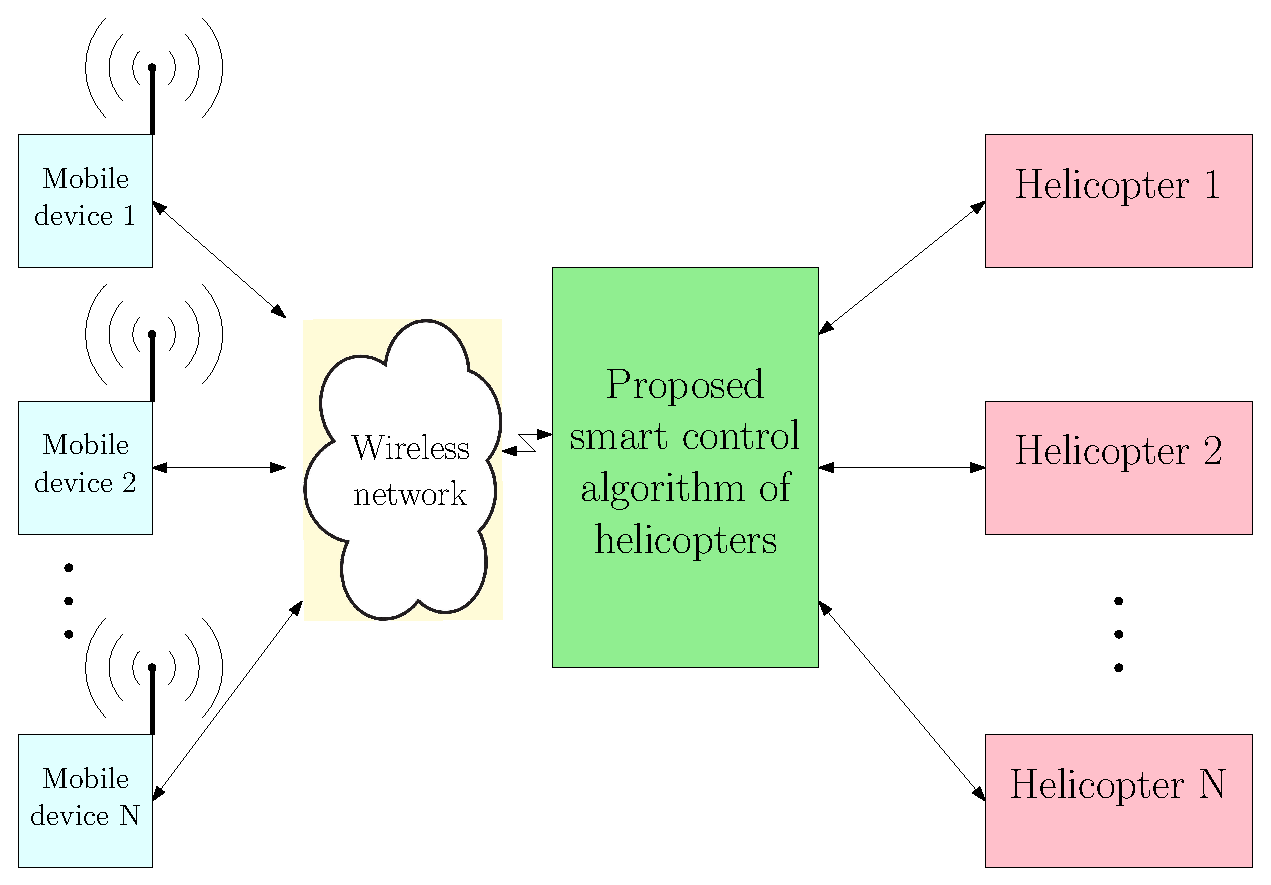
\includegraphics[scale=0.31]{figs/ipe/ProblemStatementImage}
  \end{mdframed}
  \caption{General High-Level System Architecture}
  \label{fig:ProblemStatementImage}
\end{figure}
%
In our case we will be using one mobile device and two helicopters.  Information sent by the users will be transmitted through a wireless TCP/IP network.  We will be using Raspberry Pi 3's to accomplish the wireless communication between the mobile devices and the helicopters.  Their inputs will interface with our proposed smart control algorithm and change the configuration of the helicopters.

Each of the helicopters used will have fixed bases as shown in \autoref{fig:QuanserAero} (courtesy of Quanser Inc.\footnote{\url{https://www.quanser.com/products/quanser-aero/}}). %
%
\begin{figure}
  \centering
  \includegraphics[scale=0.6]{figs/img/QuanserAero}
  \caption{Quanser Aero 2-DOF Helicopter.}
  \label{fig:QuanserAero}
\end{figure}
%
The tail of the helicopter has a motor that controls its yaw motion.  Similarly, the main rotor changes the pitch of the helicopter.  The directions in which the motors spin will be determined by the polarity of the applied voltages.  This will be regulated by our smart control algorithm.

\subsection{Proposed Smart Control Algorithm}
%system level
The system we propose for our project in \autoref{fig:ProblemStatementImage} has a mystery box with our smart control algorithm.  \autoref{fig:ProposalImage} shows our subsystem level smart control algorithm.  
%subsystem level
\begin{figure}
  \centering
  \begin{mdframed}[backgroundcolor=yellow!20, roundcorner=7pt,outerlinewidth=1.2pt,outerlinecolor=blue!50]
  \includegraphics[scale=0.335]{figs/ipe/ProposalImage}
  \end{mdframed}
  \caption{Low Level Smart Control Diagram}
  \label{fig:ProposalImage}
\end{figure}
%
This would be loaded to our Raspberry Pi 3 which is connected to the Quanser Aero, and wirelessly communicates with the mobile device.  From the mobile device you choose a desired pitch and yaw angle for your helicopters to move from their initial positions and you select a control algorithm, which is talked about later.  The algorithm selector will enable one of the three algorithms while disabling the other two.  Then the enabled algorithm takes in the desired pitch and yaw angles and the actual pitch and yaw angles, which are recorded from the helicopter, as inputs.  The actual pitch and yaw angles will also be displayed on the mobile device.  With the inputs going into the desired algorithm, voltages are calculated for each of the two motors on the helicopter to move to the desired angles. 

\subsection{Control Algorithms} % Describe LQR, LQG, and ADP
We will be using three algorithms: LQR, LQG, and ADP.

\subsubsection{LQR}
LQR (Linear Quadratic Regulator) minimizes a cost function given by the parameters \autoref{tab:aeroparameters} for the system.

The Quadratic term, \autoref{eq:matrixQ}, and Regulator term, \autoref{eq:matrixR}, are used to solve the cost function.  They are solved using algebraic Riccati equation.  Quanser proved the values shown in the matrices. 
%
\begin{align}
\label{eq:matrixQ}
Q &= 
\begin{bmatrix}
    3500 & 0 & 0 & 0 \\
    0 & 500 & 0 & 0 \\
    0 & 0 & 0 & 0 \\
    0 & 0 & 0 & 0
\end{bmatrix}
\\
\label{eq:matrixR}
R &= 0.005*
\begin{bmatrix}
    1 & 0 \\
    0 & 1
\end{bmatrix}
\end{align}
%
The steps of the LQR technique  are given in \autoref{alg:LQR-Algorithm}.
\begin{algorithm2e}
\caption{\label{alg:LQR-Algorithm} LQR Algorithm}
\DontPrintSemicolon
\Begin{
    Initialize state variable $\theta$, $\psi$, $\dot{\theta}$, and $\dot{\psi}$\;
    Initialize parameters in state-space model matrices 
    \autoref{eq:matrixA}, \autoref{eq:matrixB}, \autoref{eq:matrixC}, \autoref{eq:matrixD}\;
    Define cost function $\int_0^\infty (x^T Q x + u^T R u) dt$\;
    \Repeat{done}{
    Compute u\;
    $\bullet$~$u=ke$\; 
    $\bullet$~$e=x^d-x$\;
    $\bullet$~$\dot{e}=-\dot{x}$\;
    $\bullet$~$\dot{e}=-Ax-Bu$\;
    $\bullet$~$\dot{e}=-A(x^d-e)-Bu$\;
    $\bullet$~$\dot{e}=-Ae-Bu-Ax^d$\;
    $\bullet$~$\dot{e}=-Ae-Bke-Ax^d$\;
    Apply u to helicopter actuators
    Measure states
    }
}
\end{algorithm2e}

\subsubsection{LQG}
Once LQR is completed, we will investigate LQG (Linear Quadratic Gaussian).  This method uses a Kalman filter to eliminate noise in the system.

\subsubsection{ADP}
Once LQG is completed, we will investigate ADP (Approximate Dynamic Programming).  This method uses machine learning to optimize the system.\\
The steps of the ADP technique  are given in \autoref{alg:ADP-Algorithm}. 
\begin{algorithm2e}
\caption{\label{alg:ADP-Algorithm} ADP Algorithm}
\DontPrintSemicolon
\KwIn{${\bf x}^{[d]}$}
\KwOut{${\bf x}$}
\Begin{
    \Repeat{$t=t_f$} 
    {
    $\bullet$~$t = k\tau$\;     
    $\bullet$~Apply $u[k]$ to system model $\to x[k]$\;
    $\bullet$~Apply $\dot{x}(t)=Ax(t)+Bu(t)$ $\to x[k+1]$\;
    $\bullet$~Constrain $\psi$ on [$-180^{\circ},180^{\circ}$] and $\theta$ on [$-90^{\circ},90^{\circ}$]\;
    $\bullet$~Calculate error $\to~e[k] = x^{\text{ref}}[k] - x[k]$\;
    $\bullet$~Calculate updated $w_c$ if $t = T$\;
        \Repeat{$\Vert {w_c-w_{\text{last}}} \Vert < \epsilon_{c}$}{
        $\bullet$~$w_{\text{last}} = w_c$, $i=0$\;
            \Repeat{$i = \bar{n} - 1$}{
            $\bullet$~$u[i]=[0,0]^T$, $j=0$\;
                \Repeat{$\Vert {u[i]-u_{\text{last}}}[i] \Vert < \epsilon$ or $j=j_{\text{max}}$} 
                {
                $\bullet$~$u_{\text{last}}[i]=u[i]$\;
                $\bullet$~Find $e[i+1]$ using collected error data and $e[k+1]=f(e[k])+Gu[k]$ to $x[k]$\;
                $\bullet$~Compute new $u[i]$ using $u^*=-\frac{1}{2}R^{-1}G^T\nabla*(e(k+1))$\;
                $\bullet$~$j = j+1$\; 
                }
                \KwOut{$u[i]$}
            $\bullet$~Find $V(i)$ using $V(e(k))=e^T(k)Qe(k)+u^T(k)Ru(k)+w_C^T\phi(e(k+1))$\;
            $\bullet$~$\Lambda(i) = \phi(e(i))$\;
            $\bullet$~$i=i+1$\;            
            }
            \KwOut{$\Lambda$,$V$}
        $\bullet$~Update $w_c$ using $w_c=(\Lambda^T\Lambda)^{-1}\Lambda^-1V$\;
        } 
        \KwOut{$w_c$}
      $\bullet$~Calculate state-feedback gain using $u^*=-\frac{1}{2}R^{-1}G^T\nabla*(e(k+1))$\; and $V(e(k))=e^T(k)Pe(k)$\;
      $\bullet$~Constrain optimal inputs on [$-18,18$]\;
      $\bullet$~$k = k+1$\; 
    }    
}
\end{algorithm2e}

\subsection{Specifications}
For the proposed system, there are a few specifications that need to be met.  First, any extra materials we might need have to have an overall cost that is less than \$500 in order to stay within the budget of the department.  Second, we need to have local WiFi capabilities for the connection of the mobile device to the Raspberry Pi 3.  Third, we will be using MATLAB and Simulink to generate C code for the Raspberry Pi 3.  Finally, we will be using an Android cell phone as our mobile device for user interfacing.

\subsection{Communication Protocols}
The smart motion control algorithm runs on a single board computer which has back and forth communication between the mobile devices and the helicopter.  Fig.~\ref{fig:TCPModel} shows the overall communication structure of the current work. %
\begin{figure}
  \centering
  \includegraphics[width=0.33\textwidth]{figs/ipe/TCPModel}
  \caption{Communication model.}
  \label{fig:TCPModel}
\end{figure}
%
The mobile device running the user application sends command signals, which are then formed into a data packet to be sent over the wireless network. In this work, the user datagram protocol (UDP), which is a TCP/IP protocol, is used for the communication between the mobile device and the helicopter. It has low-latency and more tolerant to lost packets.  Next, routing information and logical addressing information are added to the packet including the internet protocol (IP) address. The link layer includes physical functions,  such as the media access control address (MAC) of the network interface card (NIC) in the packet and transmits it along a medium.  This framework utilized IEEE 802.11 which transmits the packet wirelessly through the air using radio waves.  The single board computer then removes the extraneous information until all that is left is the original data. 

\subsubsection{SPI}
SPI will be used to facilitate communication between our micro-controller (Raspberry Pi 3) and the Quanser Aero.  \autoref{tab:Embedded Wiring} contains the pin functions of the Q-flex2 embedded panel used to create the connection. \cite{quanserAeroUserManual}
\begin{table}
    \centering
    \begin{tabular}{l|l|l}
        \toprule
        \textbf{Wire} & \textbf{Color} & \textbf{Function}\\
        \toprule
        1 & White & VCC (1.8V-5V)\\
        2 & Yellow & MOSI\\
        3 & Blue & MISO\\
        4 & Green & CLK\\
        5 & Gray & QCLK (Not Used)\\
        6 & Purple & CS (Digital Output Line)\\
        7 & Red & GND\\
        \bottomrule
    \end{tabular}
    \caption{Embedded Wiring}
    \label{tab:Embedded Wiring}
\end{table}
SPI communication involves a master/slave relationship between devices.  In our case the Raspberry Pi 3 is the master device while the Aero is the slave.  What SPI allows is for the master device to send and receive data to the slave device bit by bit.  The major issue using SPI with the Quanser Aero is that SPI is meant for small quantities of data; however, the Aero sends about 51 bytes, which is not small.  Last year's group actually came up with a solution to this issue by setting the SPI clock to have a two microsecond period.


\subsubsection{Wireless}
The Raspberry Pi 3 has a network card that uses IEEE 802.11ac to be able to send and receive transmission of a wireless network.  We will use this to create a SSH connection between the Raspberry Pi and a desktop so we can interface with the terminal.  This will also be used for the communication between the Raspberry Pi and the smartphone.

\subsubsection{UDP}
UDP (User Datagram Protocol) will be used to send and receive information between the Raspberry Pi and the Android smart phone.  This is much faster than (TCP Transmission Control Protocol) because the sender and receiver do not make sure that the last transmission was received.  This is important because we want commands to be sent as quickly as possible to the Quanser and are not concerned if one out of many packets fails to be transmitted.

%----------------------------------------------------------------------------

\section{Preliminary Work}

This project is a continuation of the work done last year by Tony Birge and Andrew Fandel.  We started the lab work for this project after we had our first meeting with Dr. Miah.  We choose this project because of our interest in the field of robotics.  The following subsections contain the work we have already completed.  It includes the implementation of the LQR algorithm on one of the Quanser Aero helicopters.

\subsection{LQR Simulation Results} \label{sec:lqrsimresults}
Before we implemented LQR using a USB connection, we ran simulations in MATLAB to make sure that our algorithm would run as expected.  \autoref{fig:LQR_Error_Con} shows the position error of the pitch, yaw, speed of pitch, and speed of yaw.  \autoref{fig:LQR_Pos_Con} shows the position in degrees of the desired pitch, actual pitch, desired yaw, and actual yaw.  \autoref{fig:LQR_Volt_Con} shows the voltages applied to the motors.

\begin{figure}
  \centering
  \includegraphics[width=0.4\textwidth]{figs/matlab/LQR/LQR_Simulation/LQR_Error_Con}
  \caption{LQR Simulation Error w/ Constant Signal}
  \label{fig:LQR_Error_Con}
\end{figure}

\begin{figure}
  \centering
  \includegraphics[width=0.4\textwidth]{figs/matlab/LQR/LQR_Simulation/LQR_Pos_Con}
  \caption{LQR Simulation Position w/ Constant Signal}
  \label{fig:LQR_Pos_Con}
\end{figure}

\begin{figure}
  \centering
  \includegraphics[width=0.4\textwidth]{figs/matlab/LQR/LQR_Simulation/LQR_Volt_Con}
  \caption{LQR Simulation Voltage w/ Constant Signal}
  \label{fig:LQR_Volt_Con}
\end{figure}

\subsection{LQR USB Implementation} \label{sec:LQR_USB_imp}

Our first task that needed to be accomplished was testing and implementing the LQR algorithm onto the Aero using a USB connection.  \autoref{fig:LQR_USB} shows our Simulink model for controlling the Aero with the USB connection.  \autoref{fig:Pitch_Pos_LQR_USB_SQU} through \autoref{fig:Yaw_Volt_LQR_USB_CON} are our MATLAB implementation figures for testing different types of inputs to our model.  The inputs we used were of three types: square wave, sine wave, and constant.  We recorded the positions of both pitch and yaw angles and the voltages that were applied to the motors.

\begin{figure}
  \centering
  \includegraphics[width=0.45\textwidth]{figs/img/LQR_USB}
  \caption{LQR USB Simulink Model}
  \label{fig:LQR_USB}
\end{figure}

% Figures for Square wave with LQR USB
\begin{figure}
  \centering
  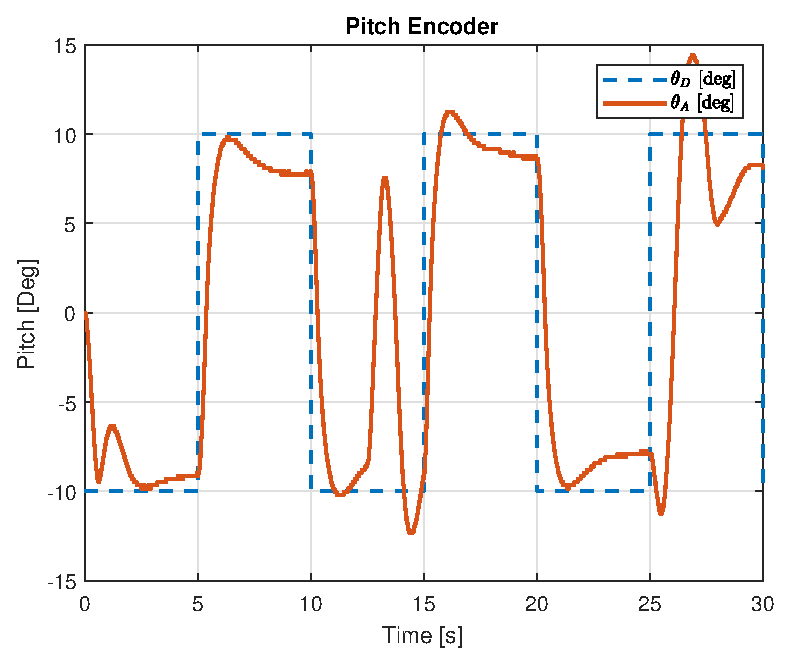
\includegraphics[width=0.4\textwidth]{figs/matlab/LQR/Pitch_Pos_LQR_USB_SQU}
  \caption{LQR USB Pitch Encoder w/ Square Wave}
  \label{fig:Pitch_Pos_LQR_USB_SQU}
\end{figure}

\begin{figure}
  \centering
  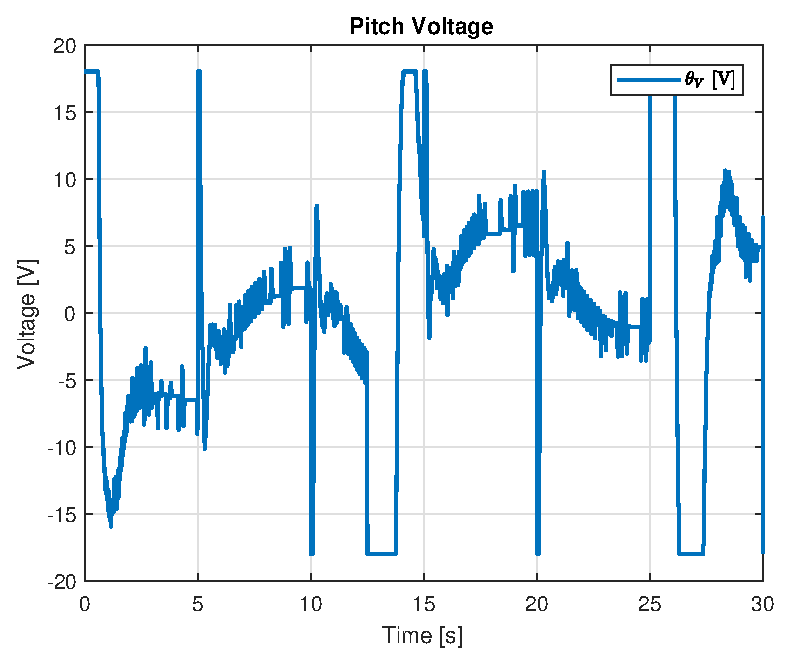
\includegraphics[width=0.4\textwidth]{figs/matlab/LQR/Pitch_Volt_LQR_USB_SQU}
  \caption{LQR USB Pitch Motor w/ Square Wave}
  \label{fig:Pitch_Volt_LQR_USB_SQU}
\end{figure}

\begin{figure}
  \centering
  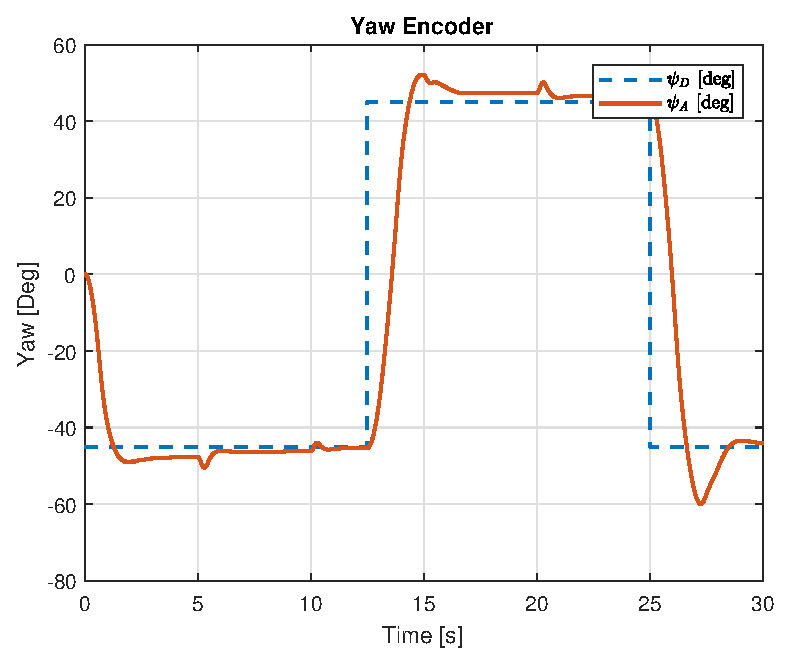
\includegraphics[width=0.4\textwidth]{figs/matlab/LQR/Yaw_Pos_LQR_USB_SQU}
  \caption{LQR USB Yaw Encoder w/ Square Wave}
  \label{fig:Yaw_Pos_LQR_USB_SQU}
\end{figure}

\begin{figure}
  \centering
  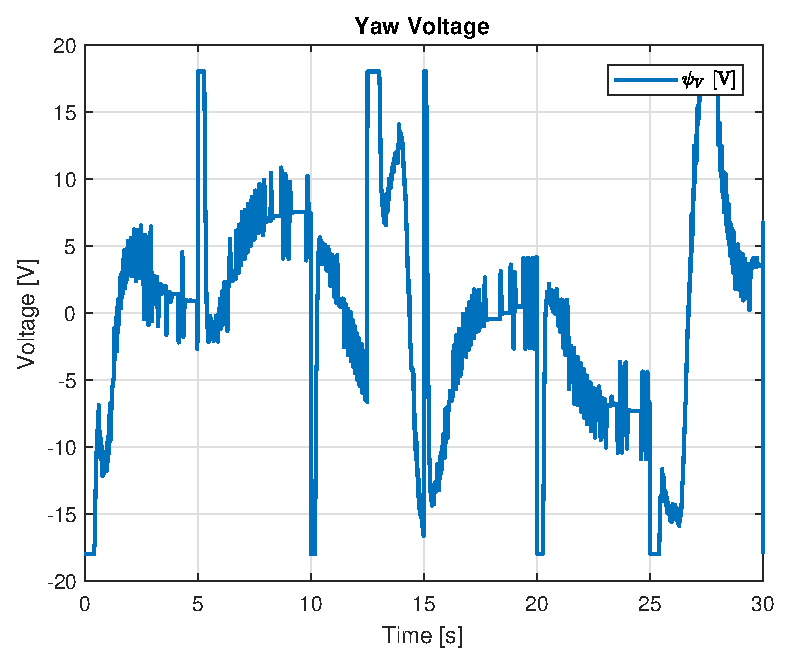
\includegraphics[width=0.4\textwidth]{figs/matlab/LQR/Yaw_Volt_LQR_USB_SQU}
  \caption{LQR USB Yaw Motor w/ Square Wave}
  \label{fig:Yaw_Volt_LQR_USB_SQU}
\end{figure}

% Sine wave figures for LQR USB
\begin{figure}
  \centering
  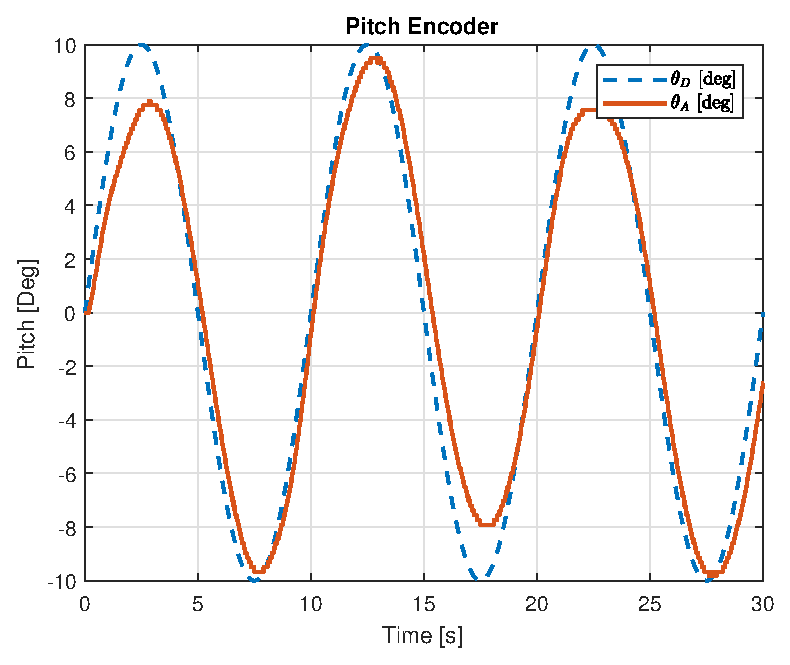
\includegraphics[width=0.4\textwidth]{figs/matlab/LQR/Pitch_Pos_LQR_USB_SIN}
  \caption{LQR USB Pitch Encoder w/ Sine Wave}
  \label{fig:Pitch_Pos_LQR_USB_SIN}
\end{figure}

\begin{figure}
  \centering
  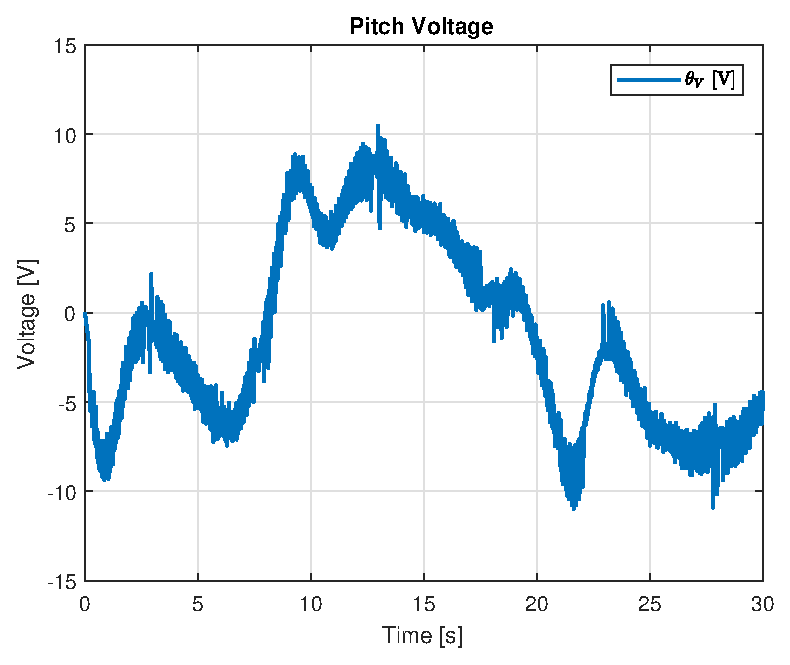
\includegraphics[width=0.4\textwidth]{figs/matlab/LQR/Pitch_Volt_LQR_USB_SIN}
  \caption{LQR USB Pitch Motor w/ Sine Wave}
  \label{fig:Pitch_Volt_LQR_USB_SIN}
\end{figure}

\begin{figure}
  \centering
  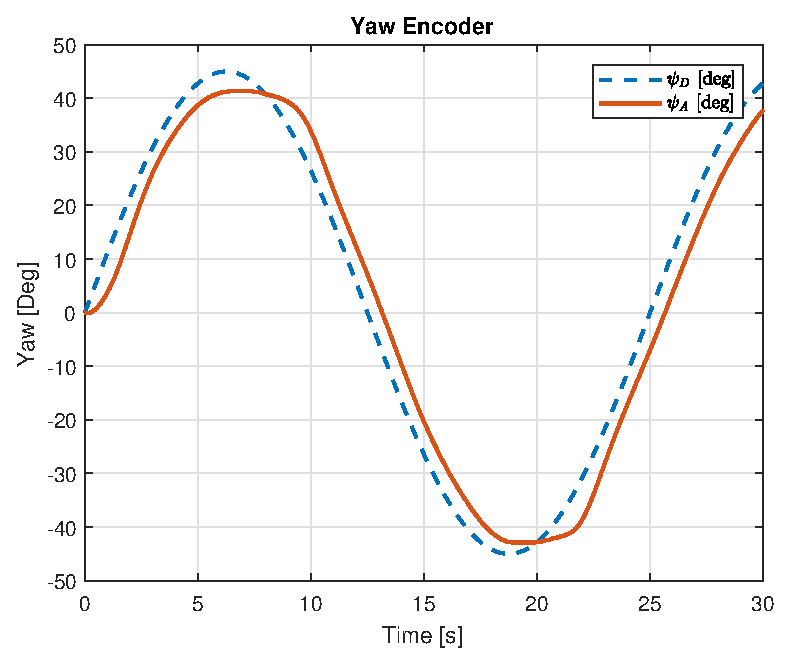
\includegraphics[width=0.4\textwidth]{figs/matlab/LQR/Yaw_Pos_LQR_USB_SIN}
  \caption{LQR USB Yaw Encoder w/ Sine Wave}
  \label{fig:Yaw_Pos_LQR_USB_SIN}
\end{figure}

\begin{figure}
  \centering
  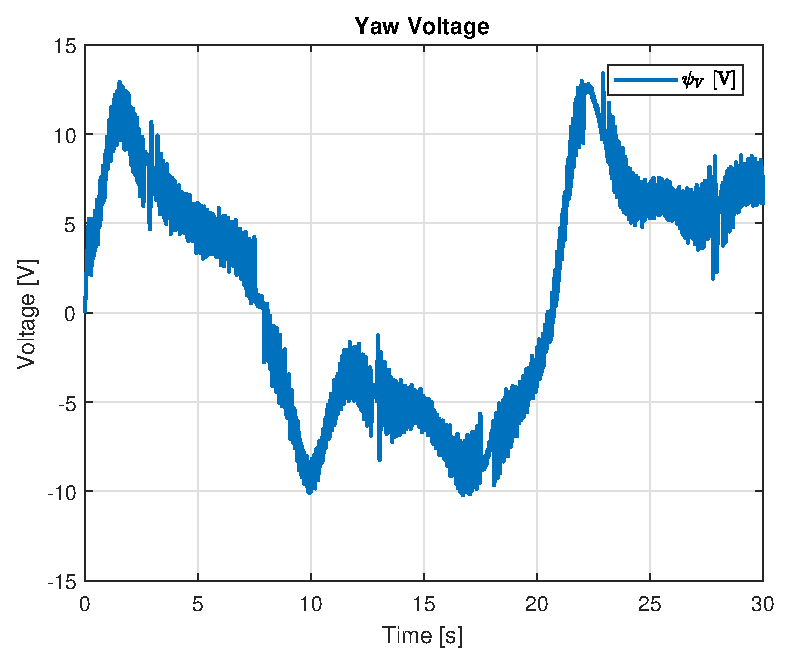
\includegraphics[width=0.4\textwidth]{figs/MATLAB/LQR/Yaw_Volt_LQR_USB_SIN}
  \caption{LQR USB Yaw Motor w/ Sine Wave}
  \label{fig:Yaw_Volt_LQR_USB_SIN}
\end{figure}

% Constant input figures for LQR USB
\begin{figure}
  \centering
  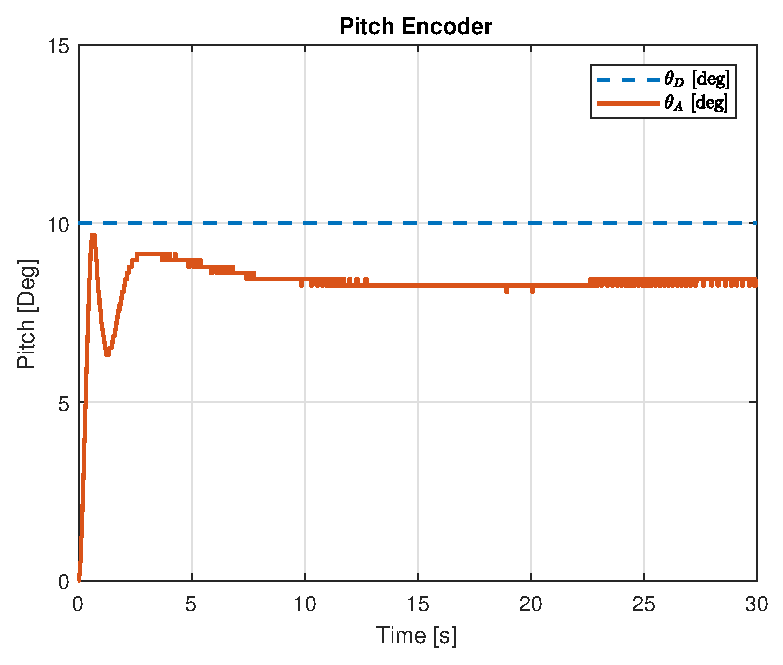
\includegraphics[width=0.4\textwidth]{figs/matlab/LQR/Pitch_Pos_LQR_USB_CON}
  \caption{LQR USB Pitch Encoder w/ Constant Input}
  \label{fig:Pitch_Pos_LQR_USB_CON}
\end{figure}

\begin{figure}
  \centering
  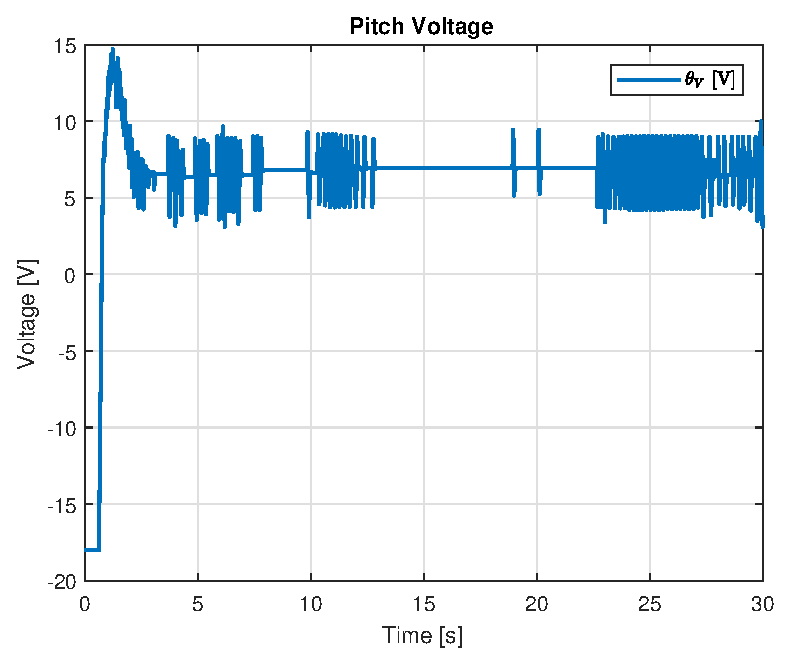
\includegraphics[width=0.4\textwidth]{figs/matlab/LQR/Pitch_Volt_LQR_USB_CON}
  \caption{LQR USB Pitch Motor w/ Constant Input}
  \label{fig:Pitch_Volt_LQR_USB_CON}
\end{figure}

\begin{figure}
  \centering
  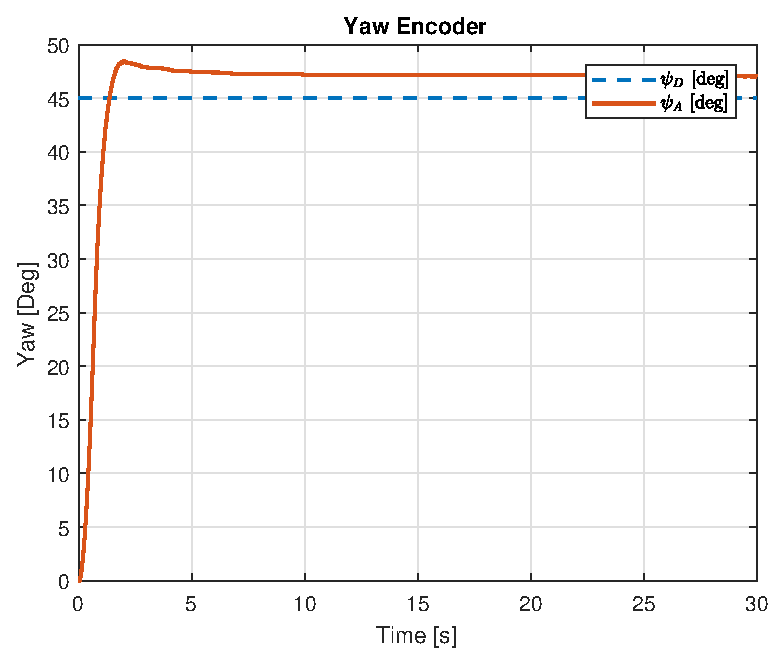
\includegraphics[width=0.45\textwidth]{figs/matlab/LQR/Yaw_Pos_LQR_USB_CON}
  \caption{LQR USB Yaw Encoder w/ Constant Input}
  \label{fig:Yaw_Pos_LQR_USB_CON}
\end{figure}

\begin{figure}
  \centering
  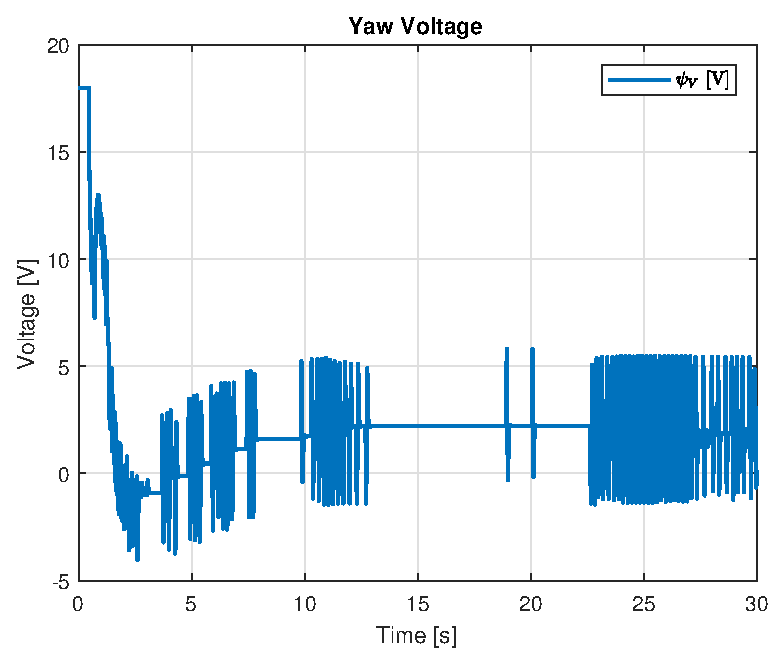
\includegraphics[width=0.45\textwidth]{figs/matlab/LQR/Yaw_Volt_LQR_USB_CON}
  \caption{LQR USB Yaw Motor w/ Constant Input}
  \label{fig:Yaw_Volt_LQR_USB_CON}
\end{figure}

\subsection{LQR Raspberry Pi Implementation} \label{sec:LQR_RPi_imp}

For using the Raspberry Pi 3 we needed to use a local network for wireless communication with the PC.  This took a little time, but we did achieve this.  Next was the issue of using SPI communication between the Raspberry Pi and the Aero.  Luckily for us, since this project is a continuation, last year's group already had a Simulink model that can implement SPI communication between the Raspberry Pi and the Aero.  After recreating every block and matching every configuration, we were able to send \autoref{fig:Basic_PI} to the Raspberry Pi 3.  \autoref{fig:SPI_COM} is the inside of the SPI Communication block in \autoref{fig:Basic_PI}.  These Simulink models are just the basic implementation of the SPI communication.  After testing it we learned a few things.  One, the initial position of the Aero is set when the Aero is started up.  Two, we need some type of user interface to be able to change the desired angles while the program is running.  That second difficulty is what we hope to be solved by the android application.

\begin{figure}
  \centering
  \includegraphics[width=0.4\textwidth]{figs/img/Basic_PI}
  \caption{Basic Top Simulink Model}
  \label{fig:Basic_PI}
\end{figure}

\begin{figure}
  \centering
  \includegraphics[width=0.4\textwidth]{figs/img/SPI_COM}
  \caption{SPI Communication Simulink Model}
  \label{fig:SPI_COM}
\end{figure}

\subsection{LQR Android Implementation} \label{sec:LQR_And_imp}

\autoref{fig:Android_LQR} is our Simulink model that will be loaded onto the Raspberry Pi 3 to control the helicopter using LQR algorithm.  For the android connectivity blocks we followed the model of last year's group.  Again, checking and rechecking all the configurations to make sure they are the same, except targeting one of our phones instead.  \autoref{fig:Android_Interface} is the Simulink model for the android application.  It will have two slider bars to set desired pitch and yaw, and will display what the actual pitch and yaw of the helicopter currently is.
%
\begin{figure}
  \centering
  \includegraphics[width=0.45\textwidth]{figs/img/Android_LQR}
  \caption{Simulink Model of LQR with Android Compatibility}
  \label{fig:Android_LQR}
\end{figure}
%
\begin{figure}
  \centering
  \includegraphics[width=0.45\textwidth]{figs/img/Android_Interface}
  \caption{Simulink Model of Phone App}
  \label{fig:Android_Interface}
\end{figure}
%
Fig.~\ref{fig:LQR_PitchVolt} and Fig.~\ref{fig:LQR_YawVolt} show the voltages that are applied to the pitch and yaw motors to move the helicopter to the configurations depicted in Fig.~\ref{fig:LQR_Pitchpos} and Fig.~\ref{fig:LQR_Yawpos}.
%
\begin{figure}
  \centering
  \subfigure[][]{
    \label{fig:LQR_Pitchpos}    
    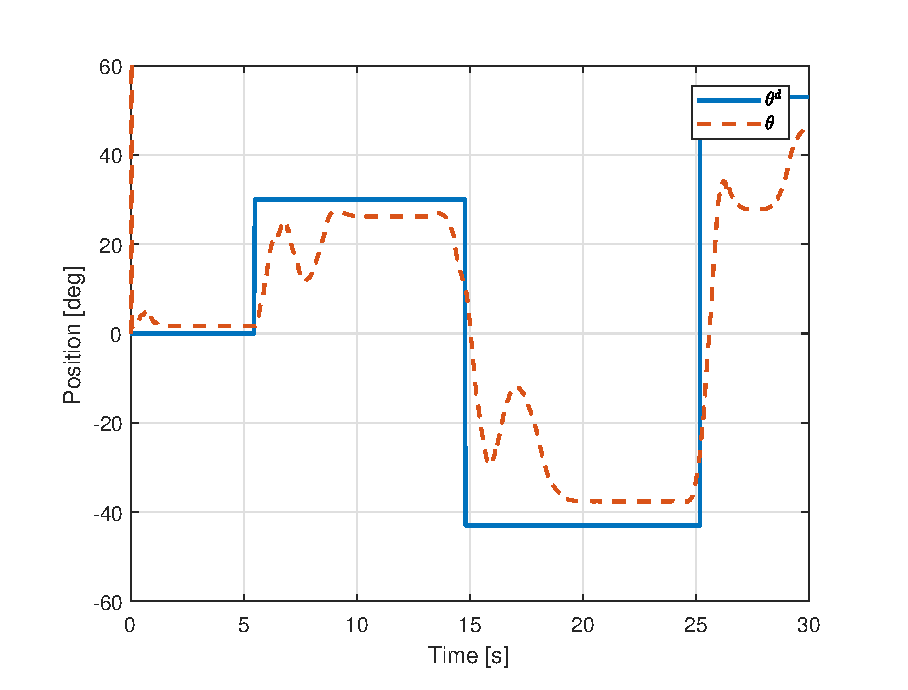
\includegraphics[width=0.33\textwidth,height=0.15\textheight]{figs/matlab/LQR/LQR_Android/LQR_Pitchpos}
  }
  \subfigure[][]{
    \label{fig:LQR_PitchVolt}
    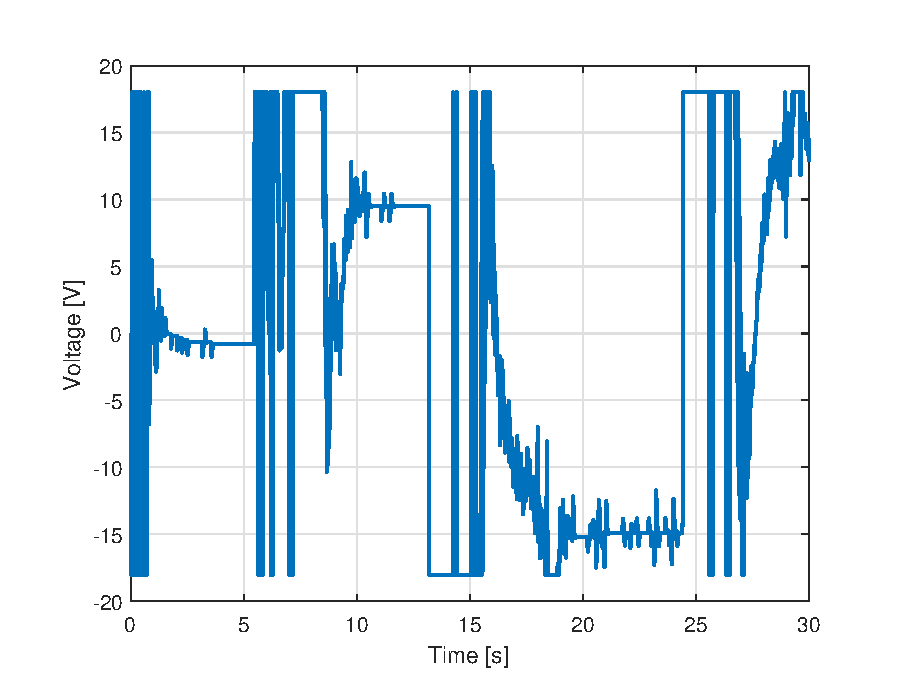
\includegraphics[width=0.33\textwidth,height=0.15\textheight]{figs/matlab/LQR/LQR_Android/LQR_PitchVolt}    
  }  
  \caption{Performance in following user's command~\subref{fig:LQR_Pitchpos} tracking pitch angle,~and~\subref{fig:LQR_PitchVolt} pitch motor input voltage.}
  \label{fig:performancePitchConst}
\end{figure}
%
\begin{figure}
  \centering
  \subfigure[][]{
    \label{fig:LQR_Yawpos}    
    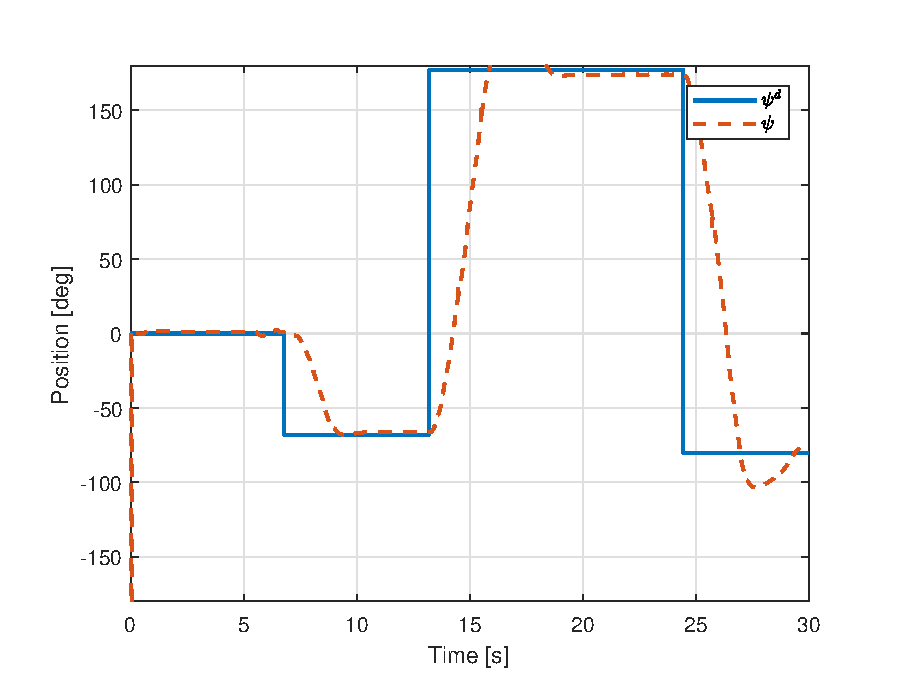
\includegraphics[width=0.33\textwidth,height=0.15\textheight]{figs/matlab/LQR/LQR_Android/LQR_Yawpos}
  }
  \subfigure[][]{
    \label{fig:LQR_YawVolt}
    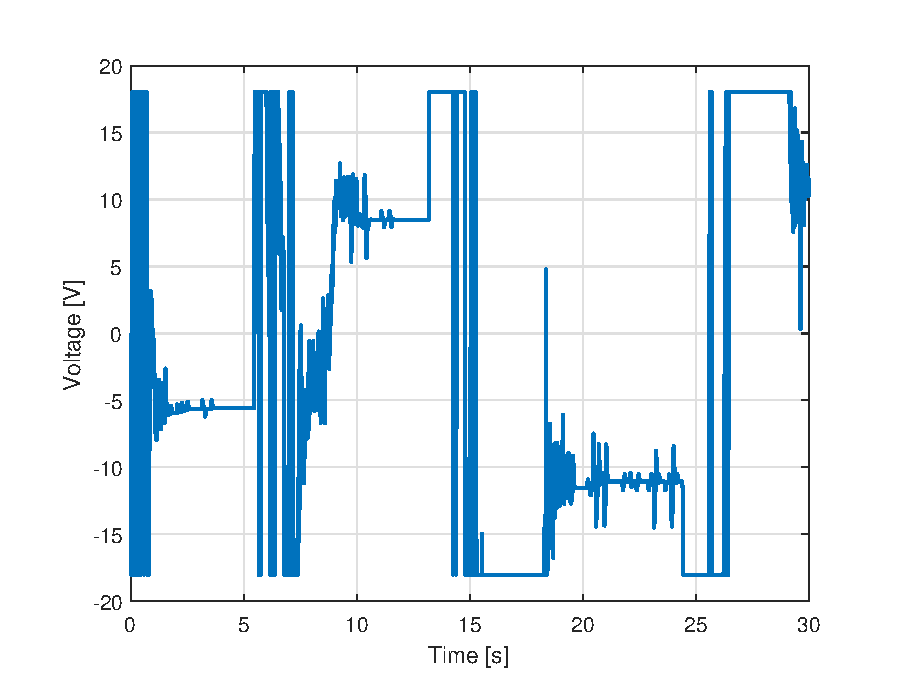
\includegraphics[width=0.33\textwidth,height=0.15\textheight]{figs/matlab/LQR/LQR_Android/LQR_YawVolt}    
  }  
  \caption{Performance in following user's command~\subref{fig:LQR_Yawpos} tracking yaw angle,~and~\subref{fig:LQR_YawVolt} yaw motor input voltage.}
  \label{fig:performanceYawConst}
\end{figure}

%---------------------------------------------------------------------------------

\section{Future Work}
Moving forward with this project, we plan on continuing with our other two algorithms.  We are in the process of simulating LQG using MATLAB.  Once this is completed, we will implement this on the Quanser Aero using USB. However, with the teaching materials that were provided to us by Quanser, we were able to implement and test an LQG algorithm that controls only pitch or yaw, but not both.  So, we are currently in the process of researching a way to couple the control for both pitch and yaw angles.  After we figure out this coupling issue and test it using the USB connection and wirelessly, we will implement LQG on an android phone.

After we complete implementing LQG all the way to the smart phone level, we will start simulating the ADP algorithm.  Like the other two algorithms we will start testing ADP using USB, then wireless communication using the Raspberry Pi.  After we get the algorithm working on the smart phone level, we will combine all three algorithms so the user may choose which algorithm they wish to use on the Aero.

%-------------------------------------------------------------------------------

\section{Parts List}
For our project, we need a two-DOF helicopter platform to incorporate our algorithms.  Bradley University acquired a Quanser Aero in 2016.  A second one was purchased in 2018.  In order to interface this platform with a micro-controller, we need a module that will facilitate communication between these two devices.  The first Aero came with a Qflex2 embedded panel as part of a promotion.  We were to convince Quanser to send us as second Qflex2 in September of 2018.

We have chosen to use a Raspberry Pi as our micro-controller.  The ECE department has several they are willing to loan out to students.  We are currently borrowing two Raspberry Pis.  In order to communicate with the Raspberry Pi using the desktop, we require a wireless network card for the PC.  The ECE department has loaned us two USB dongles for each PC.

We are also considering some add-ons to our project.  When testing, we would like to use a fan to provide some turbulence to see how each algorithm reacts.  We would also like to purchase a LCD screen that would attach to the Raspberry Pi and display the current pitch, yaw, and current algorithm.  If we progress far enough, we may be able to purchase six-DOF helicopter to implement a full range of motion.


%---------------------------------------------------------------------------------

\section{Timeline} \label{sec:timeline}
The workload for this project is split by semester.  In the Fall of 2018, \autoref{fig:gantt1}, we hope to complete LQR and LQG up to implementation on an Android phone.  In the Spring of 2019, \autoref{fig:gantt2}, we plan to complete the ADP implementation as well as testing for all three methods.

\bibliographystyle{IEEEtran}
\bibliography{bib/references.bib}

\clearpage
%\begin{figure}
\begin{sidewaysfigure}
\centering
\begin{ganttchart}[hgrid,vgrid,x unit=.5cm, y unit title=.5cm,y unit chart=.3cm,milestone label font=\tiny,bar label font=\tiny, group label font=\small,bar/.append style={fill=green},bar incomplete/.append style={fill=red}]{1}{16}
\gantttitle{2018}{16}\\
\gantttitle{Sep}{4}
\gantttitle{Oct}{4}
\gantttitle{Nov}{4}
\gantttitle{Dec}{4}\\
\ganttgroup[progress = 50,group progress label font = \tiny,progress label text={$\displaystyle#1\%$},group progress label anchor = east]{Research}{1}{14} \\
\ganttbar[progress = 100,progress label text={$\displaystyle#1\%$},bar progress label font = \tiny,bar progress label anchor = east]{Last Years Work}{1}{2}\\
\ganttbar[progress = 50,bar progress label font = \tiny,progress label text={$\displaystyle#1\%$},bar progress label anchor = east]{LQG}{3}{8}\\
\ganttbar[progress = 0,bar progress label font = \tiny,progress label text={$\displaystyle#1\%$},bar progress label anchor = east]{ADP}{9}{14}\\
\ganttgroup[progress = 50,group progress label font = \tiny,progress label text={$\displaystyle#1\%$},group progress label anchor = east]{Simulation}{1}{14}\\
\ganttbar[progress = 100,bar progress label font = \tiny,progress label text={$\displaystyle#1\%$},bar progress label anchor = east]{LQR}{1}{2}\\
\ganttbar[progress = 0,bar progress label font = \tiny,progress label text={$\displaystyle#1\%$},bar progress label anchor = east]{LQG}{3}{8}\\
\ganttbar[progress = 0,bar progress label font = \tiny,progress label text={$\displaystyle#1\%$},bar progress label anchor = east]{ADP}{9}{14}\\
\ganttgroup[progress = 100,group progress label font = \tiny,progress label text={$\displaystyle#1\%$},group progress label anchor = east]{Implementation}{3}{14}\\
\ganttbar[progress = 100,bar progress label font = \tiny,progress label text={$\displaystyle#1\%$},bar progress label anchor = east]{LQR USB}{3}{4}\\
\ganttbar[progress = 100,bar progress label font = \tiny,progress label text={$\displaystyle#1\%$},bar progress label anchor = east]{LQR Raspberry Pi}{5}{6}\\
\ganttbar[progress = 100,bar progress label font = \tiny,progress label text={$\displaystyle#1\%$},bar progress label anchor = east]{LQR Android}{7}{8}\\
\ganttbar[progress = 0,bar progress label font = \tiny,progress label text={$\displaystyle#1\%$},bar progress label anchor = east]{LQG USB}{9}{10}\\
\ganttbar[progress = 0,bar progress label font = \tiny,progress label text={$\displaystyle#1\%$},bar progress label anchor = east]{LQG Raspberry Pi}{11}{12}\\
\ganttbar[progress = 0,bar progress label font = \tiny,progress label text={$\displaystyle#1\%$},bar progress label anchor = east]{LQG Android}{13}{14}
\end{ganttchart}
\caption{Gantt chart for Fall 2018}
\label{fig:gantt1}
\end{sidewaysfigure}
%\end{figure}

%\begin{figure}
\begin{sidewaysfigure}
\centering
\begin{ganttchart}[hgrid,vgrid,x unit=.4cm, y unit title=.5cm,y unit chart=.4cm,milestone label font=\tiny,bar label font=\tiny, group label font=\small,bar/.append style={fill=green},bar incomplete/.append style={fill=red}]{1}{18}
\gantttitle{2019}{18}\\
\gantttitle{Jan}{4}
\gantttitle{Feb}{4}
\gantttitle{Mar}{4}
\gantttitle{Apr}{4}
\gantttitle{May}{2}\\
\ganttgroup[progress = 0,group progress label font = \tiny,progress label text={$\displaystyle#1\%$}, group progress label anchor = east]{Implementation}{3}{8}\\
\ganttbar[progress = 0,bar progress label font = \tiny,progress label text={$\displaystyle#1\%$},bar progress label anchor = east]{ADP USB}{3}{4}\\
\ganttbar[progress = 0,bar progress label font = \tiny,progress label text={$\displaystyle#1\%$},bar progress label anchor = east]{ADP Raspberry Pi}{5}{6}\\
\ganttbar[progress = 0,bar progress label font = \tiny,progress label text={$\displaystyle#1\%$},bar progress label anchor = east]{ADP Android}{7}{8}\\
\ganttgroup[progress = 0,group progress label font = \tiny,progress label text={$\displaystyle#1\%$}, group progress label anchor = east]{Testing}{9}{16}
\end{ganttchart}
\caption{Gantt Chart for Spring 2019}
\label{fig:gantt2}
\end{sidewaysfigure}
%\end{figure}

\end{document} 

%%% Local Variables:
%%% mode: latex
%%% TeX-master: t
%%% End:
